% !TEX TS-program = XeLaTeX
% use the following command: 
% all document files must be coded in UTF-8
\documentclass{textolivre}
% for anonymous submission
%\documentclass[anonymous]{textolivre}
% to create HTML use 
%\documentclass{textolivre-html}
% HTML compile using make4ht
% $ make4ht -c textolivre-html.cfg -u -x article "fn-in,svg,pic-align"   
%
% See more information on the repository: https://github.com/leolca/textolivre

% Metadata
\begin{filecontents*}[overwrite]{article.xmpdata}
    \Title{Drivers da adoção de metodologias não tradicionais: estudo de caso no mestrado-integrado de Engenharia Eletrotécnica e de Computadores na Universidade de Trás-os-Montes e Alto Douro, Portugal}
    \Author{Cleber Augusto Pereira \sep Paulo Moura Oliveira \sep Manuel José Cabral dos Santos Reis}
    \Language{pt-BR}
    \Keywords{Metodologias não tradicionais \sep Engenharia Eletrotécnica e de Computadores \sep Difusão da inovação \sep Teoria institucional \sep Ensino superior}
    \Journaltitle{Texto Livre}
    \Journalnumber{1983-3652}
    \Volume{14}
    \Issue{1}
    \Firstpage{1}
    \Lastpage{16}
    \Doi{10.35699/1983-3652.2021.26709}

    \setRGBcolorprofile{sRGB_IEC61966-2-1_black_scaled.icc}
            {sRGB_IEC61966-2-1_black_scaled}
            {sRGB IEC61966 v2.1 with black scaling}
            {http://www.color.org}
\end{filecontents*}



% used in this example to provide source code environment
%\crefname{lstlisting}{lista}{listas}
%\Crefname{lstlisting}{Lista}{Listas}
%\usepackage{listings}
%\renewcommand\lstlistingname{Lista}
%\lstset{language=bash,
        breaklines=true,
        basicstyle=\linespread{1}\small\ttfamily,
        numbers=none,xleftmargin=0.5cm,
        frame=none,
        framexleftmargin=0.5em,
        framexrightmargin=0.5em,
        showstringspaces=false,
        upquote=true,
        commentstyle=\color{gray},
        literate=%
           {á}{{\'a}}1 {é}{{\'e}}1 {í}{{\'i}}1 {ó}{{\'o}}1 {ú}{{\'u}}1 
           {à}{{\`a}}1 {è}{{\`e}}1 {ì}{{\`i}}1 {ò}{{\`o}}1 {ù}{{\`u}}1
           {ã}{{\~a}}1 {ẽ}{{\~e}}1 {ĩ}{{\~i}}1 {õ}{{\~o}}1 {ũ}{{\~u}}1
           {â}{{\^a}}1 {ê}{{\^e}}1 {î}{{\^i}}1 {ô}{{\^o}}1 {û}{{\^u}}1
           {ä}{{\"a}}1 {ë}{{\"e}}1 {ï}{{\"i}}1 {ö}{{\"o}}1 {ü}{{\"u}}1
           {Á}{{\'A}}1 {É}{{\'E}}1 {Í}{{\'I}}1 {Ó}{{\'O}}1 {Ú}{{\'U}}1
           {À}{{\`A}}1 {È}{{\`E}}1 {Ì}{{\`I}}1 {Ò}{{\`O}}1 {Ù}{{\`U}}1
           {Ã}{{\~A}}1 {Ẽ}{{\~E}}1 {Ũ}{{\~u}}1 {Õ}{{\~O}}1 {Ũ}{{\~U}}1
           {Â}{{\^A}}1 {Ê}{{\^E}}1 {Î}{{\^I}}1 {Ô}{{\^O}}1 {Û}{{\^U}}1
           {Ä}{{\"A}}1 {Ë}{{\"E}}1 {Ï}{{\"I}}1 {Ö}{{\"O}}1 {Ü}{{\"U}}1
           {ç}{{\c{c}}}1 {Ç}{{\c{C}}}1
}


\journalname{Texto Livre: Linguagem e Tecnologia}
\thevolume{14}
\thenumber{1}
\theyear{2021}
\receiveddate{\DTMdisplaydate{2020}{06}{08}{-1}} % YYYY MM DD
\accepteddate{\DTMdisplaydate{2020}{9}{22}{-1}}
\publisheddate{\DTMdisplaydate{2020}{12}{30}{-1}}
% Corresponding author
\corrauthor{Cleber Augusto Pereira}
% DOI
\articledoi{10.35699/1983-3652.2021.26709}
% list of available sesscions in the journal: articles, dossier, reports, essays, reviews, interviews, editorial
\articlesessionname{Ensino Superior e Tecnologia}
% Abbreviated author list for the running footer
\runningauthor{Pereira et al.}
\editorname{Leonardo Araújo}

\title{Drivers da adoção de metodologias não tradicionais: estudo de caso no mestrado-integrado de Engenharia Eletrotécnica e de Computadores na Universidade de Trás-os-Montes e Alto Douro, Portugal}
\othertitle{Drivers of the adoption of non-traditional methodologies: case study in the master- integrated of Electrical and Computer Engineering at the University Of Trás-Os-Montes and Alto Douro, Portugal}
% if there is a third language title, add here:
%\othertitle{Artikelvorlage zur Einreichung beim Texto Livre Journal}

\author[1]{Cleber Augusto Pereira \orcid{0000-0002-7704-2343} \thanks{Email: \url{al63361@utad.eu}}}
\author[1]{Paulo Moura Oliveira \orcid{0000-0003-4283-1243} \thanks{Email: \url{oliveira@utad.pt}}}
\author[1]{Manuel José Cabral dos Santos Reis  \orcid{0000-0002-8872-5721} \thanks{Email: \url{mcabral@utad.pt}}}

\affil[1]{Universidade de Trás-os-Montes e Alto Douro, Vila Real, Portugal.}

\addbibresource{article.bib}
% use biber instead of bibtex
% $ biber tl-article-template

% set language of the article
\setdefaultlanguage[variant=brazilian]{portuguese}
\setotherlanguage{english}

% for spanish, use:
%\setdefaultlanguage{spanish}
%\gappto\captionsspanish{\renewcommand{\tablename}{Tabla}} % use 'Tabla' instead of 'Cuadro'

% for languages that use special fonts, you must provide the typeface that will be used
% \setotherlanguage{arabic}
% \newfontfamily\arabicfont[Script=Arabic]{Amiri}
% \newfontfamily\arabicfontsf[Script=Arabic]{Amiri}
% \newfontfamily\arabicfonttt[Script=Arabic]{Amiri}
%
% in the article, to add arabic text use: \textlang{arabic}{ ... }

\usepackage{multirow}
\usepackage[section]{placeins}
\usepackage{rotating}

\begin{document}
\maketitle

\begin{polyabstract}
\begin{abstract}
\begin{portuguese}
O estudo analisou diversos documentos do curso de mestrado-integrado em Engenharia   Elétrica   e   de Computadores de uma Universidade Pública   Portuguesa. Avaliou-se quais são os \textit{drivers} institucionais\footnote{Para este estudo, o termo “drivers institucionais” deve ser entendido como os elementos institucionais direcionadores da adoção de metodologias não tradicionais na engenharia elétrica.} potencialmente responsáveis pela adoção de novas metodologias no curso. Realizou-se   um  estudo  de  caso com abordagem qualitativa baseada em métodos mistos: análise estatística aplicada a \textit{corpus} textuais e complementada por análise de conteúdo. Como resultados emergiram duas classes de análise de conteúdo: competências e conhecimentos esperados dos estudantes; e aspectos da formação em Engenharia Elétrica e do ciclo de estudos. Identificaram-se sete \textit{drivers} da adoção de novas metodologias no curso, com base nas teorias da difusão da inovação e teoria institucional: formação, desenvolvimento, competência, ciclo de estudos, novo, tecnologia e UC. Cada um destes \textit{drivers}  possui os seus próprios \textit{outcomes} (resultados), 16 no   total, que apresentam os efeitos percebidos pelos docentes, avaliadores de curso e coordenadores

\keywords{Metodologias não tradicionais \sep Engenharia Eletrotécnica e de Computadores \sep Difusão da inovação \sep Teoria institucional \sep Ensino superior}
\end{portuguese}
\end{abstract}

\begin{english}
\begin{abstract}
The study analyzed several instruments of the master-integrated course in Electrical and Computer Engineering at a Portuguese Public University. The institutional drivers responsible for adopting new methodologies in the course were evaluated. A case study was carried out with a qualitative approach based on mixed methods: a statistical analysis applied to textual corpus and complemented by content analysis. As a result, two classes of content analysis emerged: skills and knowledge expected from students; and aspects of training in Electrical Engineering and the study cycle. Seven drivers were identified for the adoption of new methodologies in the course, based on the theories of diffusion of innovation and institutional theory: training, development, competence, study cycle, new, technology, and UC. Each of these drivers has its outcomes, 16 in total, which shows the effects perceived by the teachers, course coordinators and evaluators.

\keywords{Non-traditional methodologies \sep Electrical and computer engineering \sep Diffusion of innovation \sep Institutional theory \sep Higher education}
\end{abstract}
\end{english}

% if there is another abstract, insert it here using the same scheme
\end{polyabstract}


\section{Introdução}\label{sec-intro}
Ao considerar a prática profissional promovida na formação superior em engenharia, \textcite{nager2016} destacaram que uma das implicações da falta de profissionais qualificados no mercado é a não adoção de novas tecnologias por parte das empresas. Isto ocorre pelo receio institucional de não conseguirem sustentar a sua aplicação ao longo do tempo, pela escassez de mão-de-obra capacitada.

\textcite{maciejewski2017} sugerem a necessidade de reforma no sistema educativo/formação de engenharia nos Estados Unidos, pois o sistema atual, na sua perspectiva, está falhando para estudantes, ex-alunos e sociedade: respectivamente pelas altas taxas de evasão, pela confusão quanto o escopo de atuação profissional entre os formados e por não atender às expectativas do mercado de trabalho. Os aspectos citados foram a pouca relevância do atual currículo associada à desatualização dos equipamentos elétricos e de informática, e o fato dos alunos finalistas em engenharia não entenderem completamente o papel de um engenheiro ou o escopo do seu campo profissional. Nesta linha, o estudo de \textcite[p. 4]{sheppard2008} foi categórico ao afirmar que “embora as escolas de engenharia visem preparar os alunos para a profissão, são influenciadas pelas tradições acadêmicas que nem sempre apoiam as necessidades da profissão”.

Seguindo a tendência de avaliar soluções aplicáveis à melhoria dos cursos de engenharia para a área de Engenharia Elétrica e de Computadores, este estudo utilizou como base de análise quatro tipos de documentos institucionais internos ou externos e de acesso público, além de entrevista aplicada ao diretor do curso de mestrado-integrado\footnote{Entenda-se como mestrado-integrado o curso de licenciatura (primeiro ciclo) seguido (integrado) do mestrado (segundo ciclo). O primeiro ciclo em Portugal é o equivalente à graduação no Brasil. O segundo ciclo em Portugal é equivalente à pós-graduação (mestrado) no Brasil.} de uma Instituição de Ensino Superior (IES) Pública em Portugal.

Este estudo tem como objetivo identificar, de forma sistemática, quais os \textit{drivers} e \textit{outcomes} institucionais que tendem a direcionar a adoção de novas metodologias no caso específico da Engenharia Elétrica e de Computadores, podendo estes achados serem objeto de teste de replicação nos demais cursos da mesma área de conhecimento. Para atingir este objetivo, recorremos à análise de forma integrada dos documentos normativos oficiais do curso de licenciatura-mestrado, dos regulamentos e normas institucionais aplicados à este, e dos resultados obtidos durante o processo de acreditação\footnote{O termo acreditação representa o processo de validação em que os cursos e programas europeus e americanos são avaliados por uma ou mais agências independentes, garantindo a transparência e impedindo ações de influência política no ensino superior. No Brasil o processo avaliativo dos cursos é de responsabilidade do Sistema Nacional de Avaliação da Edução Superior (SINAES).} pela agência reguladora, associados ao depoimento do diretor do curso.

\section{Revisão de Literatura}\label{sec-revisao}
Esta seção está organizada em duas discussões, inicialmente apresentando uma seleção das práticas aplicadas na educação em engenharia e, em seguida, uma síntese das teorias a serem adotadas no estudo.

Estudos internacionais aplicados ao ensino de engenharia têm avaliado as características, práticas e métodos adotados, relacionando-os com a qualidade da oferta e avaliação de cursos \cite{eldin2018,li2020,thibaut2018}. Estes estudos têm contribuído para a melhoria do ensino de engenharia. Há ainda estudos como os de \textcite{graham2018} e \textcite{manzoor2017} que colaboraram com o desenvolvimento de um estado-da-arte aplicável à educação em engenharia.

Numa revisão sistemática, \cite{thibaut2018} avaliaram as características e práticas adotadas na educação integrada em Ciências, Tecnologia, Engenharia e Matemática (STEM\footnote{O termo STEM provém da abreviação em inglês de \textit{'Science, Technology, Engineering, and Mathematics'}}). A estrutura proposta apresentou cinco princípios-chave a serem adotados para aumentar a escassa formação de graduados em STEM: integração de conteúdo, aprendizagem centrada no problema, aprendizagem baseada em perguntas, aprendizagem baseada em projetos e aprendizagem cooperativa. Ainda identificaram outras quatro práticas, menos frequentes, centralizadas no aluno: \textit{hands-on learning, hands-on activities and manipulatives, assessment} (da literatura anglo-saxônica), e habilidades esperadas no século 21.

O estudo de \textcite{eldin2018} reviu os documentos de quatro órgãos de controle relacionados com a formação educativa e práticas profissionais da Engenharia Elétrica. O objetivo foi identificar as práticas pedagógicas e os aspectos do processo instrucional na área. Foram relatados os resultados de experiências em universidades na Roménia e Egito, com utilização de abordagem aplicada ao Projeto. A abordagem apresentou ações de: pedagogia eletrônica para aprendizagem \textit{on-line}, \textit{e-learning} e \textit{blended learning} a serem aplicadas às práticas de ensino e aprendizagem e na formação de professores aos programas de engenharia elétrica e de computadores. Esta necessidade de adaptação do percurso de formação do engenheiro às novas práticas foi destacada por \textcite{maciejewski2017}, e o combate à tradição dos atuais professores da área foi criticada por \textcite{sheppard2008}, seja pela insistência em continuar ensinando da forma que aprenderam, desconsiderando os diferentes tempos e formas de assimilação individuais de cada aprendiz, seja pela dificuldade de adaptação às novas metodologias e práticas.

Na China, a preocupação com o desenvolvimento da engenharia e na promoção da sua adaptação ao desenvolvimento industrial no país foi debatido por \textcite{patil2007} no sentido de aumentar a competitividade internacional e adotar um modelo global de formação \cite{shuguang2019}. Um sistema de acreditação profissional é necessário para melhorar a qualidade da engenharia no país \cite{lu2019}. Na china, o termo acreditação profissional é entendido como um desafio para a melhoria das competências de engenharia dos alunos, sendo um importante critério de acreditação profissional para o ensino de engenharia a sua rápida adaptação aos novos elementos de desenvolvimento da tecnologia industrial. Além da acreditação profissional, as preocupações no país com o ensino de engenharia são inerentes aos aspectos de aderência à oferta e alcance de resultados na avaliação interna e externa dos cursos \cite{li2020}, considerando que o mercado de trabalho de engenharia da China é consideravelmente menor que o dos países desenvolvidos conforme publicado pelo Relatório de Competitividade Mundial do \textit{International Institute for Management Development}\footnote{Dados de \url{https://worldcompetitiveness.imd.org/countryprofile/CN/wcy}}.

Os estudos sobre as perspectivas profissionais da engenharia para 2020 \cite{clough2004,engineering2005,olson2016,sheppard2008} destacaram a necessidade de adaptação da profissão à economia globalizada e do ensino tornar-se mais sensível às necessidades da profissão. A luta de adaptação permeia a adoção de boas práticas e incorporação de lições aprendidas no quotidiano, sendo ainda modestas as taxas de conclusão, de permanência dos estudantes, e de participação feminina.

Ao debater o futuro da engenharia, \textcite{graham2018} sugere a entrega de uma aprendizagem autêntica e ativa a grandes grupos de estudantes. Sugere ainda o aumento da flexibilidade, escolha e diversificação, permitindo que os estudantes escolham um caminho que se adapte aos seus talentos e interesses, e a adoção de uma abordagem multidisciplinar, global e socialmente focada para os futuros engenheiros. A possibilidade de integrar e incorporar as principais experiências de aprendizagem deveriam ser incorporadas no currículo e integrar experiências como projetos de design e aprendizagem baseada no trabalho, como um caminho para os estudantes serem capazes de contextualizar e aplicar os conhecimentos e habilidades adquiridas em outras partes do currículo.

Como esclarecido no início desta seção, passa-se a apresentar os elementos fundamentais das teorias visitadas neste estudo que serão utilizadas como basilares no tratamento dos dados para avaliação dos elementos direcionadores (\textit{drivers}) da adoção de metodologias não tradicionais na engenharia elétrica. Adotou-se a Teoria do Processo de Decisão da Inovação baseada na abordagem clássica de Everett Rogers \cite{rogers1983}, e a Teoria Institucional com base na abordagem de \textcite{meyer1977}.

Na Teoria do Processo de Decisão da Inovação, \textcite{rogers1983} definiu a Difusão como o processo pelo qual uma inovação é comunicada recorrendo a canais de comunicação, ao longo do tempo, entre os membros de um sistema social. Difusão é um tipo especial de comunicação relacionada com a disseminação de mensagens que são novas ideias. A comunicação é um processo no qual os participantes criam e compartilham informações entre si, a fim de alcançar um entendimento mútuo. Um sistema social é um conjunto de unidades inter-relacionadas que estão envolvidas na solução conjunta de problemas para realizar uma tarefa comum. Um sistema possui estrutura. A estrutura é definida por \textcite{rogers1983} como arranjos padronizados das unidades num sistema, o que fornece a sua estabilidade e regularidade ao comportamento individual.

As normas são os padrões de comportamento estabelecidos para os membros de um sistema social. As normas são frequentemente exemplificadas no comportamento dos líderes de opinião num sistema, sendo subjetivas por representarem as percepções individuais sobre o que as pessoas que lhe são importantes pensam sobre a sua adoção \cite{hill1977}.

A teoria da difusão da inovação concentra-se em entender como, porquê, e, em que velocidade, as ideias e tecnologias inovadoras se propagam num sistema social \cite{rogers1983}. O processo de decisão de inovação é um processo mental no qual um indivíduo, ou outra unidade de tomada de decisão\footnote{O termo de unidade de tomada de decisão, originário do inglês \textit{Decision Making Unit} (DMU) pode representar as decisões de fechamento (aceite) de negócios, que geralmente são compartilhadas com base na avaliação de viabilidade técnica, dentre outros modelos de análise. A definição é oriunda do processo de tomada de decisão na administração e com influência da psicologia. O termo é bastante usual no processo de tomada de decisão de inovação na administração pública. É um vocábulo importado das teorias utilizadas no estudo.}, passa do primeiro conhecimento de uma inovação para formar uma atitude em relação à inovação, à decisão de adotar ou rejeitar, à implementação da nova ideia e à confirmação desta decisão \cite{davis1989,rogers1983}.

\begin{figure}[htbp]
 \centering
 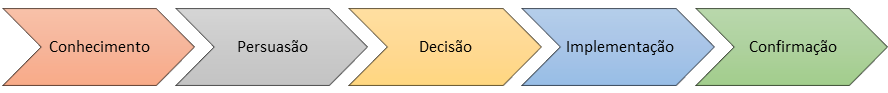
\includegraphics[width=0.5\textwidth]{Fig01.png}
 \caption{Modelo de cinco estágios no processo de decisão de inovação.}
 \label{Fig01}
 \source{Adaptado de \textcite[p. 165]{rogers1983}.}
\end{figure}

O processo de decisão de inovação ocorre em cinco estágios, estando apresentado na \cref{Fig01} como foram explicados por \textcite[p. 36]{rogers1983}:

\begin{enumerate}
\item \textit{Knowledge} (conhecimento) ocorre quando um indivíduo é exposto à existência da inovação e ganha alguma compreensão de como ela funciona;
\item \textit{Persuasion} (persuasão) ocorre quando um indivíduo forma uma atitude favorável ou desfavorável em relação à inovação;
\item \textit{Decision} (decisão) ocorre quando um indivíduo (ou outra unidade) se envolve em atividades que levam à escolha de adotar ou rejeitar a inovação;
\item \textit{Implementation} (implementação) ocorre quando um indivíduo coloca uma inovação em uso;
\item \textit{Confirmation} (confirmação) ocorre quando um indivíduo busca o reforço de uma decisão de inovação já tomada, mas ele pode reverter essa decisão anterior se exposto a mensagens conflituantes sobre a inovação.
\end{enumerate}

Para este estudo, as normas serão representadas pelos documentos do curso e institucionais. A liderança de opinião é representada pelos membros da comissão de especialistas em avaliação na ocorrência da visita para acreditação do curso\footnote{A acreditação é uma certificação profissional realizada por uma Agência externa e independente. O processo de acreditação obriga as IES a implantarem mecanismos de garantia da qualidade como a avaliação institucional que é reportada pela própria instituição e apresentada à agência de acreditação junto com as ações de controle. A agência é fiscalizada por outra agência e isto garante a independência da acreditação. Normalmente ocorre em ciclos mais longos que os processos de avaliação, e como resultado apenas fornece o status de acreditado; não acreditado; ou acreditado condicional.}, juntamente com o processo de comunicação realizado entre o curso e a agência de regulação\footnote{Apesar do termo usado oficialmente em Portugal ser “Agência de Avaliação e Acreditação do Ensino Superior” aqui utilizamos o termo “Agência de Regulação”, com o intuito de salientar o princípio “regular” que esta agência pretende ter, e que é similar ao SINAES no Brasil.}. Ao avaliar os \textit{drivers} que influenciam o processo de decisão de inovação, pode-se pontuar em que estágio do processo o curso está e direcionar a tomada de decisão, aplicando ajustes e melhorias.

Quanto à Teoria Institucional, muitas estruturas organizacionais formais surgem como reflexos de regras institucionais racionalizadas. Na sociedade moderna, tais regras são parcialmente responsáveis pela expansão e aumento da complexidade das estruturas organizacionais formais \cite{meyer1977}.

\textcite[p. 148]{dimaggio1983} destacaram que o processo de definição das estruturas organizacionais e estruturação institucional consiste em quatro partes: um aumento na amplitude da interação entre as organizações no campo; no surgimento de estruturas inter-organizacionais claramente definidas por padrões de coalizão; um aumento na carga de informação que as organizações devem lidar; e o desenvolvimento de uma consciencialização mútua entre os participantes de um grupo de organizações de que estão envolvidos num negócio comum.

\textcite{meyer1977} explicam que a força do mercado de atuação faz com que as organizações incorporem práticas e procedimentos consagrados deste mercado. As organizações que o fazem aumentam a sua legitimidade e o seu reconhecimento perante os seus pares e clientes, aumentando assim as suas possibilidades de sobrevivência, independentemente da eficácia imediata destas ações.
No seu estudo, \textcite{meyer1977} destacam que em organizações cujas estruturas se tornam isomórficas com os mitos do ambiente institucional, contrastando com aqueles estruturados principalmente pelas demandas da produção técnica e do intercâmbio, acabam por diminuir a coordenação e o controle interno para manter a legitimidade. Destacam ainda que, em alguns casos, são as próprias organizações as responsáveis por este contínuo de pessoas e processos institucionais, denominado isomorfismo.

O mecanismo de isomorfismo institucional tem uma grande influência da visão de \textcite{kanter1972} na sua discussão sobre as forças que são exercidas sobre as organizações ou comunidades, para que elas se adaptem ao mercado em que estão inseridas, passando a agir de forma semelhante ou idêntica ao mundo exterior. \textcite{meyer1977} incorporam este raciocínio, ao afirmar que quando as organizações incorporam práticas, processos e procedimentos já institucionalizados, aumentam a sua legitimidade no mercado, independentemente da eficácia, eficiência e da efetividade real desse processo de reprodução a médio e longo prazo.

\section{Metodologia}\label{sec-metodologia}
Trata-se de um estudo de caso com abordagem baseada em métodos mistos (mixed methods research). Este método é adotado na tentativa de garantir uma compreensão aprofundada pela combinação de múltiplas práticas metodológicas, diferentes materiais empíricos e diferentes perspetivas num único estudo, como estratégia para agregar rigor, complexidade, riqueza e profundidade a este estudo, tal como sugerido por \textcite{denzin2012} e \textcite{denzin2005}.

Utilizou-se um método baseado em análise estatística aplicada a \textit{corpus} textual, similar aos métodos e estudos propostos por \textcite{lebart1994}, \textcite{marchand2012}, \textcite{reinert1983} e \textcite{reinert1990}. Foi complementada por análise de conteúdo baseada em \textcite{bardin1977} e aplicada num curso de iniciativa pública em Portugal, o Mestrado Integrado em Engenharia Elétrica e de Computadores da Universidade de Trás-os-Montes e Alto Douro (UTAD).

O estudo adotou uma análise qualitativa aplicada aos seguintes relatórios:

\begin{itemize}
\item Documentos Normativos Oficiais do Curso;
\item Normativos e Regulamentos Institucionais;
\item Avaliação pela Agência de Avaliação e Acreditação do Ensino Superior (A3ES);
\item Entrevista com o Diretor do curso\footnote{Pavão, J. A. B. L. Entrevista sobre novas metodologias e tecnologias no curso de Engenharia Elétrica e de Computadores (entrevista, Outubro 3, 2017). A entrevista, na íntegra, encontra-se transcrita em documento suplementar a este texto.}.
\end{itemize}

Os dados foram cruzados para explorar o impacto das novas metodologias e tecnologias no curso de Engenharia Elétrica e de Computadores. Os documentos analisados estão apresentados na \Cref{tbl01}.

\begin{longtable}{p{0.28\textwidth} p{0.65\textwidth}}
%\begin{table}[htpb]
\caption{Documentos analisados no curso de Engenharia Elétrica e de Computadores.}
\label{tbl01}
\\
%\begin{tabularx}{\textwidth}{p{0.28\textwidth} p{0.65\textwidth}}
\toprule
\textbf{Tipos de documentos} & \textbf{Curso de Engenharia Elétrica e de Computadores de IES Pública de Portugal} \\
\midrule
Normativo do curso  & Aviso 9193/2015 que aprovou a criação do Mestrado Integrado em Engenharia Elétrica e de Computadores publicado no Diário da República (Portugal), 2ª série, nº 169 de 31 de agosto de 2015 (Universidade de Trás-os-Montes e Alto Douro - UTAD, 2015). Disponível em \url{https://bit.ly/2WtGujZ} \\
Regulamento institucional & - Regulamento Pedagógico no 136 publicado no Diário da República (Portugal), 2ª série, nº 41 de 27 de fevereiro de 2018 (UTAD, 2018). Disponível em \url{https://bit.ly/2LtGryk} \\
Avaliação pela A3ES & - Decisão do Conselho de Administração da A3ES em 15 de maio de 2015.  NCE/14/01441 – Acreditação do novo ciclo de estudos por 6 anos (Agência de Avaliação e Acreditação do Ensino Superior – A3ES, 2015a). Disponível em \url{https://bit.ly/2AvGrvD} - Relatório final da Comissão de Avaliação Externa (CAE) - NCE/14/01441 Novo ciclo de estudos (A3ES, 2015b). Disponível em \url{https://bit.ly/3eTugHB} \\
Entrevista & Realizada com o Diretor do curso. \\
\bottomrule
%\end{tabularx}
\source{dos autores.}
%\end{table}
\end{longtable}

Os dados do curso e da instituição são públicos e foram obtidos por meio de consulta ao sítio do Diário da República Portuguesa. O relatório da Agência A3ES é público e está divulgado no seu sítio institucional da Internet. A entrevista com o diretor de curso foi realizada em outubro de 2017.

% \FloatBarrier 
\subsection{Modelo de cruzamento entre o método e as teorias}\label{sec-fmt-modelo}
Para o cruzamento dos dados utilizou-se, como partida, a matriz de análise de conteúdo com uma das categorias de análise a priori validadas por \textcite{pereira2020}. Como alvo, foram utilizadas as percepções de \textit{drivers} e \textit{outcomes} estabelecidas a posteriori neste estudo, amparadas pela Teoria de Difusão da Inovações \cite{rogers1983} e pela análise de legitimidade das ações baseadas nas práticas isomórficas identificadas pela Teoria Institucional \cite{meyer1977}, revistas na \Cref{sec-revisao}.

% \usepackage{booktabs}
% \usepackage{multirow}
\begin{table}[htbp]
\caption{Modelo de cruzamento com categorias de conteúdo \textit{"a priori"} e \textit{"a posteriori"}.}
\label{tbl02}
\begin{tabularx}{\textwidth}{p{0.3\textwidth}
p{0.3\textwidth}p{0.3\textwidth}}
\toprule
\multicolumn{3}{c}{\textbf{Perceção sobre metodologias não-tradicionais}} \\ 
\midrule
\multicolumn{3}{c}{Subcategorias – a priori} \\ 
\midrule
Formas associadas ao termo “metodologias não-tradicionais” &
Diferenciação entre metodologia do Projeto Pedagógico e metodologia específica de cada Unidade Curricular (UC) &
  Adoção de metodologias não-tradicionais diferentes perspetivas \\ \midrule
\end{tabularx}

\begin{tabularx}{\textwidth}{p{0.48\textwidth}
p{0.48\textwidth}}
\multicolumn{2}{c}{\textbf{Análises a posteriori}} \\ \midrule
Base documental e entrevista:\newline
\begin{itemize}
    \item \textbf{Normativo do curso};
    \item \textbf{Regulamento} Institucional;
    \item \textbf{Avaliações} pela Agência de Regulação;
    \item \textbf{Relato} do diretor de curso.
\end{itemize} &
Quem são os \textit{Drivers}?\newline Como são percebidos pelos  \textit{Outcomes}? \newline
\begin{itemize}
    \item Docentes;
    \item Unidades curriculares;
    \item Ciclo de estudos.
\end{itemize} \\
\bottomrule
\end{tabularx}
\source{Adaptado de \textcite{pereira2020}.}
\end{table}

As quatro dimensões de documentos definidos na \cref{tbl01} (Normativos do curso, Regulamentos Institucionais, Avaliação realizada pela A3ES, e Entrevista com o Diretor de curso) foram integradas no modelo de análise cruzada proposto na \cref{tbl02} e formaram o \textit{corpus} textual de análise.

\subsection{Critérios e métodos aplicados ao \textit{corpus} textual dos relatórios}\label{sec-criterios}
Durante a preparação do \textit{dataset} as palavras compostas de todo o \textit{corpus} textual foram conectadas por \textit{underlines} para garantir sua representação dentro do contexto e realizar seu processamento. Por exemplo, o termo “ciclo de estudos” foi padronizado como “ciclo-de-estudos”. Em contrapartida, para estas ocorrências não foi possível realizar a análise léxica e utilização de sinônimos destes vocábulos, por não existirem equivalência de termos compostos no dicionário de dados do software utilizado para este processamento\footnote{Como ferramenta de produtividade foi utilizado o software Iramuteq no tratamento e análise dos dados.}. 
Todo o \textit{corpus} textual teve de ser adaptado e revisado antes de seu processamento, eliminando os símbolos e espaços entre parágrafos, dentre outros requisitos. O objetivo da padronização do \textit{corpus} textual foi de qualificar seus elementos utilizando categorias lexicais e/ou semânticas e quantificá-las, ao analisar a composição e frequência de ocorrência dos seus elementos textuais.

Para as análises, utilizou-se como termos ativos os adjetivos, substantivos, verbos e as palavras compostas anteriormente explicadas. As demais categorias foram marcadas como suplementares para efeito de evitar repetições de termos não significativos e poluição visual. Tanto os termos ativos como suplementares são considerados nos Segmentos de Texto (ST) não gerando qualquer prejuízo aos extratos textuais de todo o corpus.  

O \textit{corpus} textual processado apresentou 8.436 ocorrências de palavras em 306 ST, com uma média de 27,57 palavras por ST, contendo, ao total, 1.837 palavras distintas que constituem o vocabulário textual desta análise. Destas, 1.344 foram formas lematizadas distintas, 1.130 na forma ativa e 205 formas suplementares. A relação entre as formas ativas que apresentaram frequências maiores que 3 foi de 418. Ocorreram 594 palavras únicas, os hápax.

Ainda como método, calculou-se a riqueza do vocabulário utilizado nesta análise. Este foi baseado numa simplificação da Lei de Zipf \cite{booth1967,zipf1949} que foi uma das precursoras no tratamento estatísticos de textos escritos. \textcite{zipf1949} observou a existência de um padrão de comportamento na distribuição de palavras num texto, ao transformar esse texto em unidades lexicais e ordená-las de acordo com sua frequência de ocorrência decrescente, observando que o produto da ordem de série pela frequência é uma constante (C) para cada texto analisado, representada pela expressão (1), em que r representa a ordem de classificação e f a frequência de ocorrências no texto:
\begin{equation}
r \times f = C,
\end{equation}

Foi aplicada ao \textit{corpus} textual a Classificação Hierárquica Descendente (CHD). Adotou-se o método de \textcite{reinert1990}, pelo fato do estudo exigir uma análise conjugada de conteúdo de relatórios de diversificadas fontes, no sentido de obter classes originadas por palavras que são significantes associadas com aquela classe. \textcite[p. 187]{reinert1983} destacou ser “muito raro ter inicialmente um conjunto de indicadores confiáveis que possam ser assimilados a variáveis”. Isto deve-se ao fato de não sabermos, a priori, o significado que ela assume em determinado subconjunto de dados, devido à necessidade de considerar o contexto.

A CHD permite agrupar os indicadores polissêmicos em classes características de determinados contextos. O processamento dos \textit{clusters} foi realizado à posteriori, segundo o método proposto por \textcite{reinert1990}, obtendo uma retenção de 79,08\% de todo o \textit{corpus} textual, aproveitando 242 ST do \textit{corpus} textual inicial de 306 ST, o que foi considerado adequado para a análise a ser realizada.

Para apresentação das classes de análise de conteúdo foi utilizado o Dendrograma de Classes, elaborado com base na Análise Fatorial de Correspondência (AFC), que associou textos dos relatórios com as modalidades de contexto, possibilitando a comparação dos conteúdos destas modalidades por classe. Nesta análise, foi possível identificar um número pequeno de fatores que puderam ser usados para identificar variáveis inter-relacionadas como definido por \textcite{lebart1994}.

\section{Resultados da análise}\label{sec-resultados}
No decorrer desta seção serão apresentados os resultados das seguintes análises. Começou-se pelo cálculo da riqueza do vocabulário utilizado, que é uma medida confirmatória da relevância do papel do \textit{corpus} textual para o estudo, continuou-se apresentou-se um ranking dos principais termos segundo a Lei de \textcite{zipf1949}.

Depois, apresentam-se os resultados da Classificação Hierárquica Descendente (CHD) com o processamento das 5 classes de análise de conteúdo que emergiram do \textit{corpus} textual. A representação das classes foi evidenciada pelo Dendrograma de classes, como apresentação gráfica das características de cada agrupamento. O Dendrograma foi elaborado com base nos resultados da Análise Fatorial Confirmatória (AFC), fornecendo as variáveis representativas do contexto de cada agrupamento.

Em seguida utilizou-se a Análise de Similaridade (ADS) juntamente com a nuvem de palavras como \textit{modus operandi} para detalhar e explicar as características de cada classe. 

Adotou-se o padrão de apresentar, após a explicação individual de cada classe, os potenciais \textit{drivers} e \textit{outcomes} da adoção de metodologias não tradicionais.

Por fim, apresenta-se o mapeamento consolidado dos achados no curso com as suas representações na ADS. 

\subsection{Riqueza do vocabulário analisado e ranking dos termos segundo a Lei de Zipf}\label{sec-riqueza}
A riqueza lexical do vocabulário é uma medida estatística, uma relação que se estabelece entre o número de palavras repetidas e diferentes de um texto e o número total de palavras nele encontradas \cite{sardinha2008}. Neste estudo, a riqueza lexical do vocabulário foi de 21,78\%, calculada pela razão entre o número de formas distintas (1.837) e o número total de ocorrências de palavras (8.436).

Considerou-se adequada esta medida, tendo em conta a recorrência de palavras importantes em seu respectivo contexto. Um extrato sintético das palavras, e as suas recorrências no \textit{corpus} textual, é evidenciado na \cref{tbl03}.


\begin{table}
\caption{Aplicação da Lei de Zipf nos documentos de Engenharia Elétrica e de Computadores.}
\label{tbl03}
%\small
%\hskip-0.45cm
\noindent\adjustbox{max width=0.92\textwidth}{%
\begin{tabularx}{\textwidth}{llllllll}
\rowcolor[HTML]{4472C4} 
\multicolumn{1}{|l|}{\cellcolor[HTML]{4472C4}Palavras(f)} & Rank (r) & Freq.(f) & rf(C) & Palavra(f) & Rank(r) & Freq. (f) & rf(C) \\ \rowcolor[HTML]{B4C6E7} 
Estudante              & 2  & 70 & 140 & Avaliação contínua    & 41  & 15 & 615  \\
\rowcolor[HTML]{D9E2F3} 
Avaliação              & 3  & 54 & 162 & Plano de estudos      & 44  & 15 & 660  \\
\rowcolor[HTML]{B4C6E7} 
Docente                & 5  & 44 & 220 & Unidades curriculares & 57  & 14 & 789  \\
\rowcolor[HTML]{D9E2F3} 
Ciclo de estudos       & 8  & 35 & 280 & Mestrado-integrado    & 64  & 12 & 768  \\
\rowcolor[HTML]{B4C6E7} 
Científico             & 16 & 24 & 384 & Metodologia           & 89  & 10 & 890  \\
\rowcolor[HTML]{D9E2F3} 
Elementos de avaliação & 30 & 18 & 540 & Estrutura curricular  & 176 & 6  & 1056
\end{tabularx}
}
\source{dos autores.}
\end{table}

Pela aplicação simplificada da lei de \textcite{zipf1949} realizou-se a ordenação por frequência de ocorrências, permitindo ser observada uma relação entre este ordenamento na forma de ranking e a frequência de cada ocorrência. Note-se que algumas destas terminologias suportam ou representam consensos da área, podendo assumir a forma de potenciais \textit{drivers} da adoção de novas metodologias. Esta aplicação pode ser vista na Tabela 3, destacando-se os termos “estrutura curricular”, “ciclo de estudos” e “unidades curriculares”. No contexto do ES brasileiro, estes termos são homônimos à “grade curricular”, categoria de curso: “graduação ou pós-graduação” e “disciplinas”.

Ainda na \Cref{tbl03} 3 é evidenciado um extrato com alguns vocábulos que se destacaram durante a análise por apresentarem elevada frequência ou \textit{rank} significativos de ocorrência no \textit{corpus} textual. A Tabela 3 está ordenada por (C) em ordem crescente. Nota-se, por exemplo, que os termos “estrutura curricular” e “metodologia” se destacaram na amostra, impulsionados pelo alto \textit{rank} (r) associados à frequência de repetição (f), sendo termos que podem obter importante destaque para a riqueza lexical do vocabulário. Nesta lógica, os termos “plano de estudos”, “avaliação contínua” e “elementos de avaliação” também podem ser potenciais destaques para a análise da adoção de metodologias não tradicionais no curso avaliado.

\subsection{Resultados da Classificação Hierárquica Descendente pelo método de Reinert}\label{sec-classificacao}
\textcite{lebart1994}explicam que durante a análise de conteúdo feita à posteriori, o investigador identifica as ocorrências ao longo do \textit{corpus} textual a ser analisado e num segundo momento, realiza a contagem e construção de cada uma dessas categorias que sistematizam a análise.

Para isto, realizou-se primeiro a Classificação Hierárquica Descendente (CHD), utilizando-se do procedimento sugerido por \textcite{reinert1990} e validado estatisticamente por \textcite{benzecri2007}. O procedimento consistiu em dividir o \textit{corpus} textual em classes temáticas homogêneas de acordo com as palavras ou conceitos que contêm. A CHD revela as estruturas temáticas do texto \cite{reinert1990}. Estas estruturas foram apresentadas pela visualização em nuvem de palavras específicas de cada classe. A CHD ocorre por iterações sucessivas a partir de uma análise fatorial das correspondências múltiplas \cite{benzecri2007}.

Em seguida foi feita a composição das classes temáticas, definida a nomenclatura individual adequada para cada uma, caracterizando seu conteúdo através da análise das ocorrências de Segmentos de Textos (ST) e frequência de ocorrência das formas.
O \textit{corpus} textual aproveitado para a criação das classes obteve 6.660 ocorrências de palavras em 1.175 formas distintas. Apresentou 544 palavras distintas, os hápax com 8,17\% das ocorrências e 46,3\% das formas. No final do processamento foram geradas 5 classes distintas em dois grandes agrupamentos. Estas serão explicadas a partir do Dendrograma de classes apresentado na próxima seção.

\subsubsection{Dendrograma de classes}\label{sec-dendrograma}
O primeiro agrupamento foi formado pelas Classe 5 e Classe 2 que são complementares entre si por tratarem da formação promovida pelo curso de Engenharia Elétrica e de Computadores:

\begin{itemize}
\item Classe 5 – aspectos da formação em Engenharia Elétrica e do ciclo de estudos;
\item Classe 2 – Competências e conhecimentos esperados dos estudantes.
\end{itemize}

O segundo agrupamento foi formado pelas Classes 1, 4 e 3. Destas, as Classes 3 e 4 são semelhantes e versam sobre os processos de controle e de garantia da qualidade aplicados no curso. A Classe 1 é uma especialização das Classes 4 e 3, apresentando as minúcias relativas aos métodos de avaliação associados aos critérios normativos institucionais e do curso. Foram assim denominadas:

\begin{itemize}
\item Classe 1 – Métodos e critérios de aprovação;
\item Classe 4 – Controle pedagógico pelos serviços académicos (regras);
\item Classe 3 – Garantia da qualidade.
\end{itemize}

Usando a proposta de \textcite{reinert1990} foi possível recuperar o contexto em que as palavras ocorreram, passando a considerar na análise, além do vocabulário, os ST em que o vocabulário estava inserido, contribuindo para a fidedignidade das interpretações. A análise foi realizada por ordem de variáveis, aqui representadas pelas ocorrências de palavras com maior frequência de evocação no \textit{corpus} textual. O critério de corte utilizado foi a consideração de, no mínimo, cinco repetições de cada palavra.

Para a construção do Dendrograma das classes (\cref{Fig02}) foi realizada a Análise Fatorial de Correspondência (AFC). A AFC possibilitou identificar um número relativamente pequeno de fatores que puderam ser usados para apontar relações entre variáveis, podendo identificar variáveis inter-relacionadas.

\begin{figure}[htbp]
 \centering
 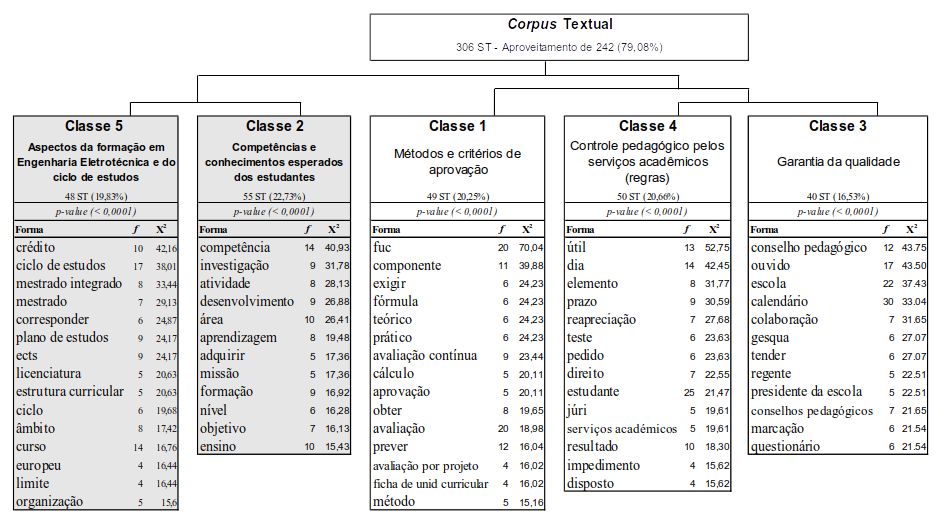
\includegraphics[width=0.85\textwidth]{Fig02.png}
 \caption{Dendrograma de classes.}
 \label{Fig02}
 \source{dos autores.}
\end{figure}

O resultado final é a representação pelo Dendrograma de Classes (\Cref{Fig02}), apresentando a coleção simultânea de várias variáveis em torno de um mesmo objeto, a classe \cite{lebart1994}. Para separação das classes verificou-se a proximidade entre as palavras, assim como suas distâncias e relevância dentro das suas divisões. Os termos mais fortes de cada classe são destacados. A composição das classes, as suas características e excertos serão apresentadas na próxima seção.

\subsection{Explicação das Principais Classes do Estudo}\label{sec-explicacao}
Nesta seção serão explicadas como foram compostas as Classes 2 e 5, marcadas com preenchimento escuro no Dendrograma de Classes da \cref{Fig02} e, após a explicação de cada uma, apresentam-se seus potenciais \textit{drivers} e \textit{outcomes} e a sua vinculação com as teorias da decisão da inovação e da teoria institucional. Estas classes foram selecionadas pela afinidade de seu conteúdo com o estudo proposto.

\subsubsection{Classe 2 – Competências e conhecimentos esperados dos estudantes}\label{sec-classe}
A Classe 2 “Competências e conhecimentos esperados dos estudantes” destacou as formas “competência”, “investigação”, “atividade”, “desenvolvimento”, “adquirir” e “aprendizagem”, todas com p significativo (< 0,0001).

\begin{figure}[htbp]
 \centering
 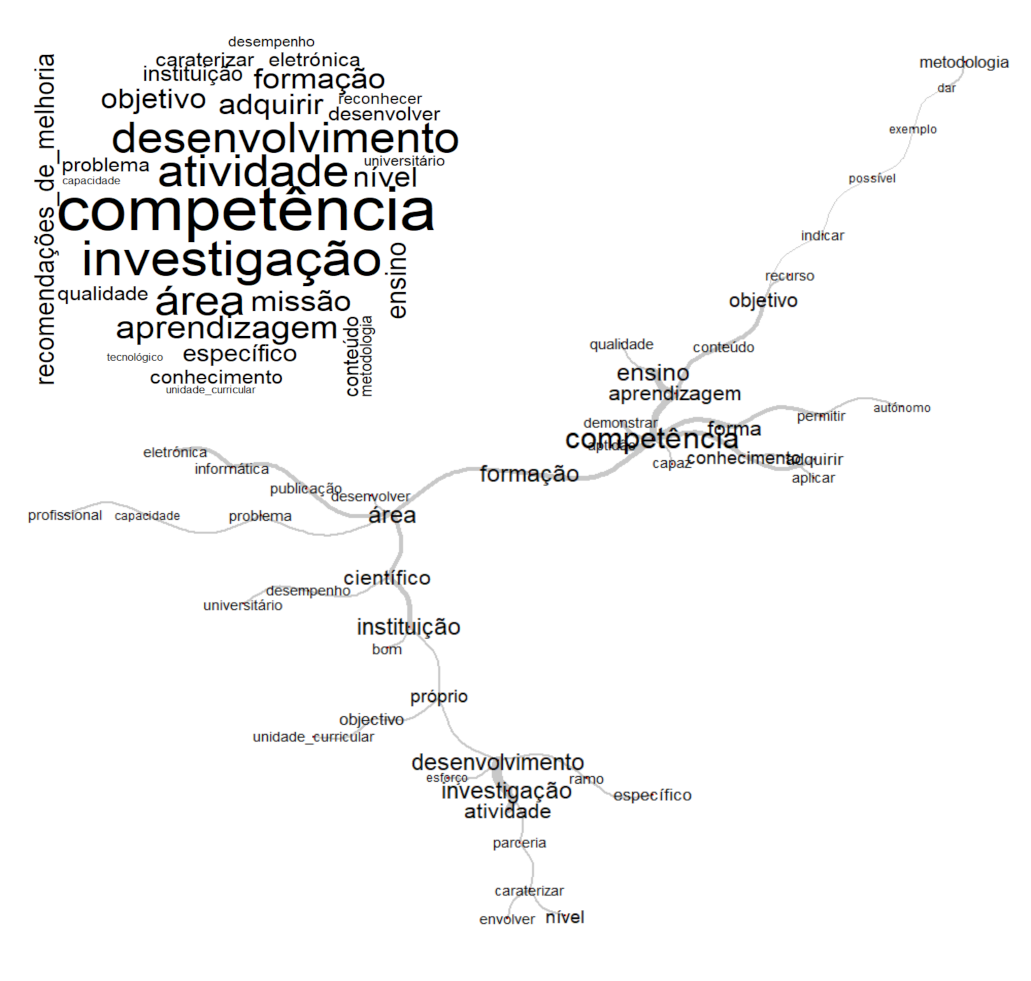
\includegraphics[width=0.85\textwidth]{Fig03.png}
 \caption{Classe 2 “Competências e conhecimentos esperados dos estudantes”.}
 \label{Fig03}
\source{dos autores.}
\end{figure}

O termo “competência”, apresentou χ2 (qui-quadrado) de 31,78, o maior da classe, ocorrendo em 14 ST. O termo “investigação”, χ2 de 40,93; ocorreu em 9 ST. “Atividade” obteve χ2 de 28,13, em 8 ST e “desenvolvimento”, χ2 de 26,88 ocorrendo em 9 ST na classe.

A Análise de Similaridade da Classe 2, combinada com a sua respectiva nuvem de palavras, é apresentada na Figura 3. 
Na \cref{Fig03}, são detalhadas as conexões entre os principais termos através das linhas e espessuras destas linhas para representar a força entre as conexões do \textit{corpus} textual e a sua proximidade, apresentando-se na forma de um grafo. Nesta análise é possível inferir a estrutura de construção do texto, pois foram construídas considerando a estrutura dos parágrafos (ST) e destacam os temas de relativa importância, a partir da coocorrência entre as palavras. Para a construção do grafo da \cref{Fig03}, assim como das demais classes a serem apresentadas, foram criados supcorpora específicos, para garantir as conexões e características individuais de cada classe.

Destacou-se nesta Classe a forte influência da “formação” de “competências” nos estudantes. Ativada devido ao desenvolvimento de atividades de “ensino-aprendizagem” de elevado nível de “conhecimento” proporcionando um bom “desempenho científico” nos universitários. São destacados os termos referenciados no parágrafo anterior que atuam como raízes centrais de forte ligação com os outros termos.

Neste cerne, o termo “competência” é uma raiz central que se associou mais fortemente com as outras raízes de menor força de coocorrência, mas não menos importantes, como: “ensino-aprendizagem”, “área” + “profissional” e “desempenho” + “científico” + “tecnologia”. Embora estes termos sejam elementos centrais da representação, as suas ramificações permitem-nos inferir a estreita ligação destes para o alcance do resultado final esperado dos estudantes: as competências do engenheiro. Isto pode ser destacado nos excertos:

\begin{quote}[...] demonstrar \textbf{competências de aprendizagem} que lhes permitam prosseguir os estudos para aprender quer individualmente quer em grupo de forma autónoma e ao longo de toda a sua vida ativa  *

[...] para além disso independentemente do percurso de especialização os mestres deverão demonstrar conhecimento e \textbf{competências avançadas na área da electrotecnia} capazes de constituir a base de desenvolvimentos e ou aplicações originais em muitos casos em contexto de investigação  *

[...] revelar capacidade de análise e concepção ao nível da aplicação do conhecimento de modo a resolver problemas em situações novas em contextos alargados e multidisciplinares com \textbf{competência} profissional *

[...] ser capazes de fundamentar os seus raciocínios e conclusões com argumentação própria de forma clara e concisa demonstrar \textbf{competências de aprendizagem ao longo da vida} que lhes permitam evoluir profissionalmente de forma autónoma*
* Regulamento Institucional \cite[grifo nosso]{utad2018}
\end{quote}

A nuvem de palavras destacou os termos com maior frequência de ocorrência na Classe, as palavras são apresentadas com tamanhos distintos porque as maiores são aquelas que detêm maior importância e coocorrência.

Os excertos e os termos potenciais destacados aqui irão compor a discussão dos \textit{drivers} e \textit{outcomes} apresentados na próxima seção.

\textbf{Discussão dos \textit{Drivers} e \textit{Outcomes} da adoção de metodologias não tradicionais da Classe 2}

Como potenciais drivers para adoção de metodologias não tradicionais nesta classe temos: “competência”, “desenvolvimento” e “formação”. Os \textit{drivers} podem ser entendidos como indicadores de meios que têm a capacidade de mostrar a tendência de adoção no curso.

Os \textit{outcomes} funcionam como indicadores dos resultados induzidos pelos \textit{drivers}. Aqui os potenciais candidatos a \textit{outcomes} de metodologias não tradicionais que estão ligados às “competência”, “desenvolvimento” e “formação”:

\begin{itemize}
\item “Competência” = “adquirir” + “desenvolver”, “ensino” + “aprendizagem”;
\item “Desenvolvimento” = “desempenho” + “investigação”;
\item “Formação” = “conhecimento” + “científico” + “tecnológico” + “unidade curricular”.
\end{itemize}

Apresenta-se a seguir os excertos que fundamentam a proposição, os \textit{drivers} estão destacados em negrito e \textit{outcomes} estão destacados em itálico, quando mencionados no texto.

\begin{quote}
[...] actividades de \textbf{formação} e investigação, existe um Centro de Investigação em que os docentes \textbf{desenvolvem} a sua atividade científica, reconhecido e com boa avaliação na área predominante do ciclo de estudos *

[...] a avaliação se destina a apurar os conhecimentos e as \textbf{competências} adquiridas pelos estudantes constituindo uma atividade pedagógica indissociável do processo de ensino aprendizagem *

[...] ser capazes de fundamentar os seus raciocínios e conclusões com argumentação própria de forma clara e concisa demonstrar \textbf{competências} de \textbf{aprendizagem} ao longo da vida que lhes permitam evoluir profissionalmente de forma autónoma* 		
	* Regulamento Institucional (\cite{utad2018}, grifo nosso)
\end{quote}

Note-se que o nó da raiz representado por “competência” é o principal direcionador dos demais \textit{drivers}, neste caso aplicada ao “ensino” + “aprendizagem” e às ações de “adquirir” e/ou “desenvolver” (competências). O nó da raiz “formação” representa o \textit{driver} dos aspectos relativos a “conhecimento” + “científico” dos estudantes. O nó “desenvolvimento” é o principal direcionador (\textit{driver}) das diretivas (\textit{outcomes}) “desempenho” em “investigação”.

Os excertos que se destacaram neste sentido foram os que ressaltam a preocupação dos docentes em reconhecer o seu status quo, o que não significa vantagem individual. Como observado por \textcite{rogers1983} isto pode afetar a percepção individual dos membros de um sistema social sendo geradora de caos e podendo afetar a validade das normas deste sistema.

Ao avaliar as competências adquiridas pelos discentes durante a sua formação é desejado pelo mercado de trabalho a capacidade de demonstração do conhecimento dos egressos de forma autónoma durante a sua atividade profissional.

Como o processo de decisão de inovação é um processo mental, os \textit{drivers} “competência”, “desenvolvimento” e “formação” parecem atuar no curso, alocados no quarto estágio, o de implementação. Ao isolar os ruídos do status quo nos docentes, ou seja, diminuindo a exposição a produção de mensagens conflitantes sobre a inovação, a tendência é a ocorrência de um avanço de estágio, na direção da confirmação, o último estágio do processo de decisão da inovação. Nisto o curso passa a reforçar a decisão de inovação anteriormente tomada, no sentido de consolidação destes \textit{drivers} como difusores da inovação.

\subsubsection{Classe 5 - Aspectos da formação em Engenharia Elétrica e do ciclo de estudos}\label{sec-aspectos}
A Classe 5 “aspectos da formação em Engenharia Elétrica e do ciclo de estudos”, destacou na AFC as formas “crédito”, “ciclo de estudos”, “mestrado-integrado”, “plano de estudos”, “licenciatura” e “mestrado”, todas com p significativo (< 0,0001): “crédito”, com χ2 de 42,16 o maior da classe, ocorrendo em 10 ST que contêm a palavra na classe; “ciclo de estudos”, com χ2 de 38,01 ocorreu em 17 ST na classe; e “mestrado-integrado”, com χ2 de 33,44 ocorrendo em 8 ST na classe.

Os achados desta classe podem ser considerados confirmatórios dos \textit{drivers} selecionados na Classe 2. Funcionam como uma especialização da Classe 2. Por exemplo, “plano de estudos”, “licenciatura” e “mestrado” são uma especialização de “ciclo de estudos” que foi classificada como \textit{driver} nesta Classe. Também ficou legitimado que o “ciclo de estudos” é “realizado” pela oferta de um conjunto de “unidades curriculares”.

Os excertos típicos desta classe permeiam a noção derivada da teoria institucional, justificando o fato de a instituição incorporar práticas isomórficas e procedimentos consagrados no mercado educacional, com o objetivo de aumentar a sua legitimidade e o seu reconhecimento perante os seus \textit{stakeholders}, numa tentativa de estender as suas possibilidades de sobrevivência perante o processo de acreditação pela agência de regulação, independentemente da eficácia imediata destas ações. Alguns excertos que demonstram os ST típicos da classe são apresentados a seguir. Consideram-se excertos típicos, os trechos que comportaram grande quantidade de formas em um mesmo parágrafo ou ST.

\begin{quote}
\textbf{A estrutura curricular} e \textbf{plano de estudos cumprem} os requisitos legais e como \textbf{mestrado-integrado} no \textbf{âmbito} da \textbf{engenharia eletrotécnica e de computadores} é solução corrente em várias \textbf{instituições} universitárias \textbf{europeias} **

o \textbf{ciclo de estudos} tem objetivos de aprendizagem análogos às de outros \textbf{projetos educativos} de \textbf{instituições} de \textbf{referência} do espaço europeu de ensino \textbf{superior} **   

o \textbf{ciclo de estudos} tem duração e estrutura semelhantes a \textbf{projecto educativo} de \textbf{instituições} de \textbf{referência} do espaço \textbf{europeu} de ensino \textbf{superior} **      

** avaliação pela Agência de Regulação (\cite{A3ES2015a}; \cite{A3ES2015b}, grifo nosso)
\end{quote}

A Análise de Similaridade (ADS) da Classe 5, combinada com sua respectiva nuvem de palavras, é apresentada na Figura 4. 

Nela ficam evidenciados os principais nós representados pelos termos “ECTS”, “curso”, “crédito”, “mestrado-integrado” e, como principal, o “ciclo de estudos”.

Cada nó apresenta as suas ramificações, que foram construídas com base no texto principal, organizado por parágrafos, os ST. 

Fica evidenciado na ADS que as suas características detalham a maioria dos aspectos inerentes ao percurso de formação promovido pelo curso.

\begin{figure}[htbp]
 \centering
 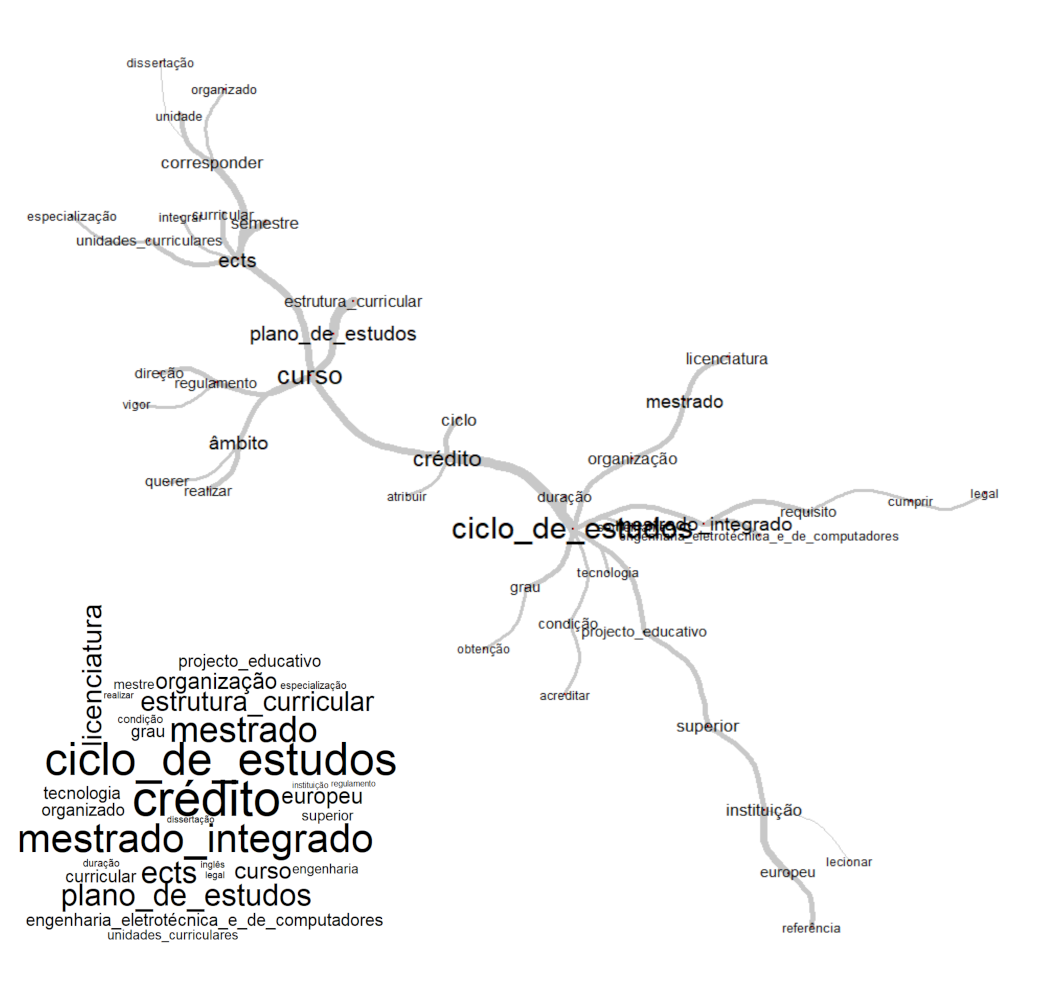
\includegraphics[width=0.5\textwidth]{Fig04.png}
 \caption{Classe 5 “aspectos da formação em Engenharia Elétrica e do ciclo de estudos”.}
 \label{Fig04}
 \source{dos autores.}
\end{figure}

Esta classe, na sua origem, foi formada prioritariamente por relatos oriundos da avaliação realizada pela Agência de Regulação do Ensino Superior no país, a A3ES, e por fragmentos do relato do diretor de curso, em sua entrevista.

\textbf{Discussão dos \textit{Drivers} e \textit{Outcomes} da adoção de metodologias não tradicionais da Classe 5}

Esta classe, em contraste, apresentou características fortemente institucionais no sentido de um sistema social estruturado na forma de ciclo de estudos, uma licenciatura seguida de mestrado, como estabelecido por \textcite{rogers1983}.

Tem uma estrutura formada por arranjos organizacionais padronizados nas suas subunidades: “estrutura curricular”, “plano de estudos”, “objetivos de aprendizagem” e “requisitos legais”, num sistema com uma composição teórica derivada da teoria de isomorfismo institucional.

Isto pode ser facilmente evidenciado quando os excertos relatam as práticas adotadas pelo curso serem semelhantes às adotadas por outros cursos como “a estrutura curricular e plano de estudos cumprem os requisitos legais e [...] é solução corrente em várias instituições universitárias europeias” \cite{A3ES2015a}, e seguido pela afirmação da comissão de especialistas em avaliação destacando que “o ciclo de estudos tem duração e estrutura semelhantes a projecto educativo de instituições de referência do espaço europeu de ensino superior” \cite{A3ES2015b}.   

Estas características destacadas de isomorfismo institucional, como explicado por \textcite{dimaggio1983}, são identificadas ao adotar práticas, regras e/ou normas, ou modelos de trabalho que já estejam institucionalizados, conduzindo o curso da instituição a agir de forma semelhante ou idêntica aos concorrentes.

No relato do diretor do curso, apresentaram-se evidências de decisão de inovação, nas falas em que cita o processo mental, como um desejo individual de inserir duas inovações:  escrita académica em inglês; e, a escrita das dissertações tanto em inglês como em português, como nos excertos (grifo nosso):

\begin{quote}
[...] mas é uma coisa \textbf{nova} que eu \textbf{quero} introduzir e que ainda não consegui até agora que é a \textbf{escrita em inglês} desde o primeiro \textbf{ano} ***

Eu \textbf{queria} que as \textbf{dissertações do mestrado} pudessem ser feitas como previsto na lei, \textbf{quer} em \textbf{inglês, quer} em português ***
*** relato do Diretor do curso
\end{quote}

Foi possível identificar o estágio em que anda este processo na decisão de inovação: numa fase de transição entre a “persuasão” e a “decisão”\footnote{Ver o detalhe dos estágios do processo de decisão da inovação apresentados na \cref{Fig01}} \cite{rogers1983}. O discurso do diretor observou\footnote{As características do segundo estágio, “Persuasão”, foram apresentadas na revisão de literatura.} as vantagens relativas e a compatibilidade destas duas ações para o curso, mas ainda não passou para o estágio de “decisão” através da comunicação ao corpo docente para formar uma atitude em relação à inovação, garantindo o atendimento à complexidade da decisão de avaliar a possível adoção ou rejeição da nova ideia pela equipa.

Nas evocações do diretor fica evidente o \textit{driver} “novo”, caracterizado pela persuasão de inovação, mas com o fator de adoção limitado parcialmente pela idade do corpo docente. Neste cerne, o termo “novo” teve como \textit{outcomes} o “âmbito” de “querer” e “realizar” no contexto de novas tecnologias. Já o \textit{driver} “tecnologia” apresentou os seus \textit{outcomes} no contexto do “projecto educativo”. Os excertos que seguem fundamentam estas afirmações (destaque nosso):

\begin{quote}
[...] claro que sim, o nosso corpo docente está a envelhecer, mas eu acho que ainda há \textbf{espaço} para a introdução de \textbf{novas tecnologias} por uma parte deles ***

[...] eu creio que eles seriam capazes de fazer pequenas experiências, e que fossem alargando, a medida dos resultados destas \textbf{novas experiências}. Resistência sim, oposição acredito que não. Eles não teriam grandes problemas se tivermos o cuidado de explicar o que está a passar ***
*** relato do Diretor de curso
\end{quote}

Por último, a Ficha de Unidade Curricular (FUC\footnote{Este é um caso em que a FUC, embora não esteja vinculada diretamente à classe em discussão, apresentou nesta classe repercussões da sua capacidade de direcionar \textit{outcomes}, por isto, foi incluída desde já como um driver, embora seja identificada como um elemento direto da Classe 1.}) demonstrou ser um \textit{outcome} da dinâmica do \textit{driver} “UC” mediando e avaliando as ações pedagógicas no curso e avaliando o que funciona e o que não funcionou em cada semestre letivo como relatado pelo Diretor de curso (grifo nosso): “ele\footnote{Referindo-se à Ficha de Unidade Curricular (FUC).} é \textbf{correspondente} ao \textbf{semestre}, mas é dinâmico e vai refletindo o que funcionou ou não”.

Destaque-se ainda que a forma “unidades curriculares” (no plural) e “UC”, embora apareçam no diagrama separadas, representam evocações unitárias de “UC” na forma completa e abreviada; isto acontece devido ao contexto em que foram evocadas no \textit{corpus} textual. Portanto, “UC”, “Ficha de Unidade Curricular”, e “FUC”, embora tenham sido classificadas na Classe 1, que não foi objeto de discussão, por apresentar um dos maiores valores de χ2 (70,039), provou ser um elemento essencial da dinâmica do ensino, devendo ser aqui considerado.

O mesmo acontece com o termo associativo próximo a estas duas formas: “realizar”, com 3 evocações e “realização”, com 4 evocações.

As demais classes (1, 4 e 3) não apresentaram características ou excertos que as permitissem serem enquadradas nas abordagens deste estudo. Os seus respectivos conteúdos demonstraram-se predominantemente procedimentais e prescritivos, não colaborando com o propósito de adoção de metodologias não tradicionais no curso, facto pelo que não serão aqui detalhados.

\section{Mapeamento dos \textit{Drivers} e \textit{Outcomes} da Adoção de Metodologias não Tradicionais}\label{sec-mapeamento}
Durante o estudo puderam ser identificados sete \textit{drivers} e dezessete \textit{outcomes} a estes associados, como fatores influentes no processo de adoção de metodologias não tradicionais no curso de Engenharia Elétrica e de Computadores. Estes achados foram organizados e classificados no sentido de manter as suas interdependências, além de evidenciar a sua associação (χ2) entre os elementos nas classes.  

A Tabela 4 apresenta a síntese dos \textit{drivers} e \textit{outcomes} com as suas respectivas classificações por classe. Os três primeiros \textit{drivers} “Formação”, “Desenvolvimento” e “Competência” foram representativos da Classe 2. Mostraram-se associados à transição entre o quarto e o quinto estágio do processo de decisão da inovação, entre a implementação e a confirmação da sua decisão de inovação.

A formação é outro \textit{driver} que teve como \textit{outcomes} a unidade curricular e as iniciativas de realização com caráter de fornecer conhecimento científico e tecnológico. A formação é apoiada pelos \textit{outcomes} das Tecnologias utilizadas na Engenharia Elétrica e de Computadores e encontra-se no processo de transição para a confirmação, o quinto estágio do processo de decisão da inovação.

As competências são um \textit{driver}, que pode ser medido pelos \textit{outcomes} que aferem o seu estado de pleno desenvolvimento institucional, sendo adquiridas no processo de ensino e de aprendizagem, como foram apresentadas na Classe 2 (grifo nosso):

\begin{quote}
[...] independentemente do percurso de especialização os mestres deverão \textbf{demonstrar conhecimento e competências} avançadas na \textbf{área} da electrotecnia \textbf{capazes} de constituir a base de \textbf{desenvolvimentos} e ou aplicações originais em muitos casos em contexto de \textbf{investigação}

de \textbf{forma} individual e em equipa no âmbito da \textbf{área} de \textbf{formação} de \textbf{competências} que lhes \textbf{permitam} comunicar informação ideias \textbf{problemas} e soluções aos vários públicos
\end{quote}

O desenvolvimento é um driver caracterizado pela forte atuação em investigação que reflete o alto desempenho do curso. Neste item específico, a rede de investigação compartilhada entre centros de investigação associados com outras instituições reconhecidas no cenário do ensino superior europeu, favorece a internalização das melhores práticas institucionais isomórficas. Estes resultados permitem o posicionamento estratégico do curso como semelhante aos demais cursos de engenharia de referência no espaço europeu.

Em seguida “Ciclo de Estudos”, “Novo” e “Tecnologia” representam a Classe 5.

O “Ciclo de estudos” foi o driver que demonstrou ter como outcomes os aspectos da formação científica dos estudantes, referenciado através da realização de um conjunto de diversas unidades curriculares organizadas: “Quanto à estrutura do ciclo de estudos, [...] o mestrado integrado inclui uma componente curricular constituída por um conjunto organizado de unidades curriculares a que correspondem 258 ECTS” \cite[parág. 5]{utad2015}. Apresentou características de adoção de práticas isomórficas de legitimação do curso perante a comunidade académica, científica e pelos utilizadores, principalmente destacado pela avaliação da A3ES quando o associou aos cursos de referência no espaço europeu de ensino superior.

O \textit{driver} “Novo” representa o desejo do diretor de curso avançar com a persuasão entre os integrantes do curso e promover a decisão de adoção de inovação. O estágio atual é o intermediário entre a persuasão e a decisão de adoção.

A tecnologia é o \textit{driver} que permeou o projecto educativo como um arranjo organizacional padronizado baseado na replicação das práticas já consolidadas no meio académico, estando consolidado num isomorfismo institucional.

Como exceção, mas não menos importante, “UC” foi oriundo da Classe 1, mas com grande representatividade na sua relação com a “Ficha de Unidade Curricular” e “FUC” através dos valores significativos do seu χ2 e grande recorrência no \textit{corpus} textual. Isto deve-se ao entendimento de ser o documento instrucional mais significativo na operacionalização de cada UC. A UC pode ser considerada um \textit{driver} operacional juntamente com a utilização da Ficha de Unidade Curricular e FUC, elementos documentadores e dinâmicos, das iniciativas individuais adotadas pelos docentes. Os outcomes da FUC relatam a realização das ações nas unidades curriculares (UCs). Por isto, é a principal evidência da existência de mecanismos de controle institucionais com adoção de regras, normas e modelos isomórficos semelhantes aos definidos por outros cursos de referência.

\begin{table}[!t] %Manter assim para melhor alinhamento - João 13/01/24
	\centering
	\small
	\begin{threeparttable}
		\caption*{\textbf{Exemplo 3.}}
		\label{tab-04}
		\begin{tabular}{@{} 
				>{\raggedright\arraybackslash}p{(\columnwidth - 2\tabcolsep) * \real{0.0300}} 
				>{\raggedright\arraybackslash}p{(\columnwidth - 2\tabcolsep) * \real{0.9700}} @{}}
			\toprule\noalign{}
			\multicolumn{2}{l}{Milton Santos: compreensão de aula de LP}  \\
			\midrule\noalign{}
			
			\multirow{6}{*}{\textbf{1ª}}   & \textbf{64. MS:} porque as minhas aulas de português são:: ficam \emph{meio chata} por quê? porque é só aquele negócio \emph{leitura e escrever leitura e escrever} entendeu? (...) \\
			
			&\textbf{65. KA: }sim \\
			
			&\textbf{66. MS: }aí isso vai dando uma preguiça da aula que (...) \\
			
			&\textbf{67. KA: }é verdade \\
			
			&\textbf{68. MS: }não tem nada diferente \emph{nunca tem nada diferente} é \emph{só ler e escrever ler e escrever} e\ldots{} \\
			
			&\textbf{217. MS:} sim basicamente \emph{usou só} livro podemos se dizer \\
            \midrule
			
			\multirow{3}{*}{\textbf{2ª }} & \textbf{148. MS:} SIM::: juro foi o que eu mais gostei de todo essa trajetória de vocês aqui...porque geralmente no ensino ... tradicional ... \emph{o ensino tradicional costuma dá... a questão e a resposta}... já na pesquisa de vocês estivemos que \emph{ir atrás da resposta}... não foi dada de mão beijada... e eu gostei pois \emph{desafiava a gente}... aquela coisa toda... \emph{a gente compreendia melhor} ... olha eu usando o a gente {[}...{]} \\
			
			&\textbf{165. KA:} você participaria de outra pesquisa como essa ... que a gente desenvolveu? \\
			
			&\textbf{166. MS:} SIM::... inclusive eu já iria falar ...\emph{se outra pesquisa dessa acontecesse atualmente ... nossa eu me empenharia  muito mais}... por que assim... vocês chegaram com a pesquisa ... no momento que eu tava... tão sabe... então em toda a pesquisa tava tendo um esforço a triplo pra fazer todas as coisas... agora atualmente ... eu digo que minha base de conhecimento ...aumentou um pouquinho pelo menos...e que é melhor em uma pesquisa \\
			
			\bottomrule
		\end{tabular}
	\end{threeparttable}
\centering
\end{table}


A \Cref{tbl04} apresenta individualmente cada \textit{driver} seguido pelos seus \textit{outcomes} correspondentes. Destacam-se ainda na (\cref{tbl04}) os valores individuais dos seus χ2 em cada classe. O objetivo é sintetizar os achados do estudo e apresentar um resumo de cada elemento potencial, associando as suas ligações internas com os seus outcomes, e referenciando sempre a sua classe originária.

A \cref{Fig05} apresenta, de forma sistemática e consolidada, os \textit{drivers} e \textit{outcomes} que emergiram da classificação realizada neste estudo. Durante toda esta análise, pela realização da análise léxica das palavras, estas foram reduzidas ao singular e ao gênero masculino, fato que elucida a apresentação no diagrama dos termos “novo” + “tecnologia” que é equivalente a “novas tecnologias”, dentre outras situações semelhantes e pontuais.

\begin{figure}[htbp]
 \centering
 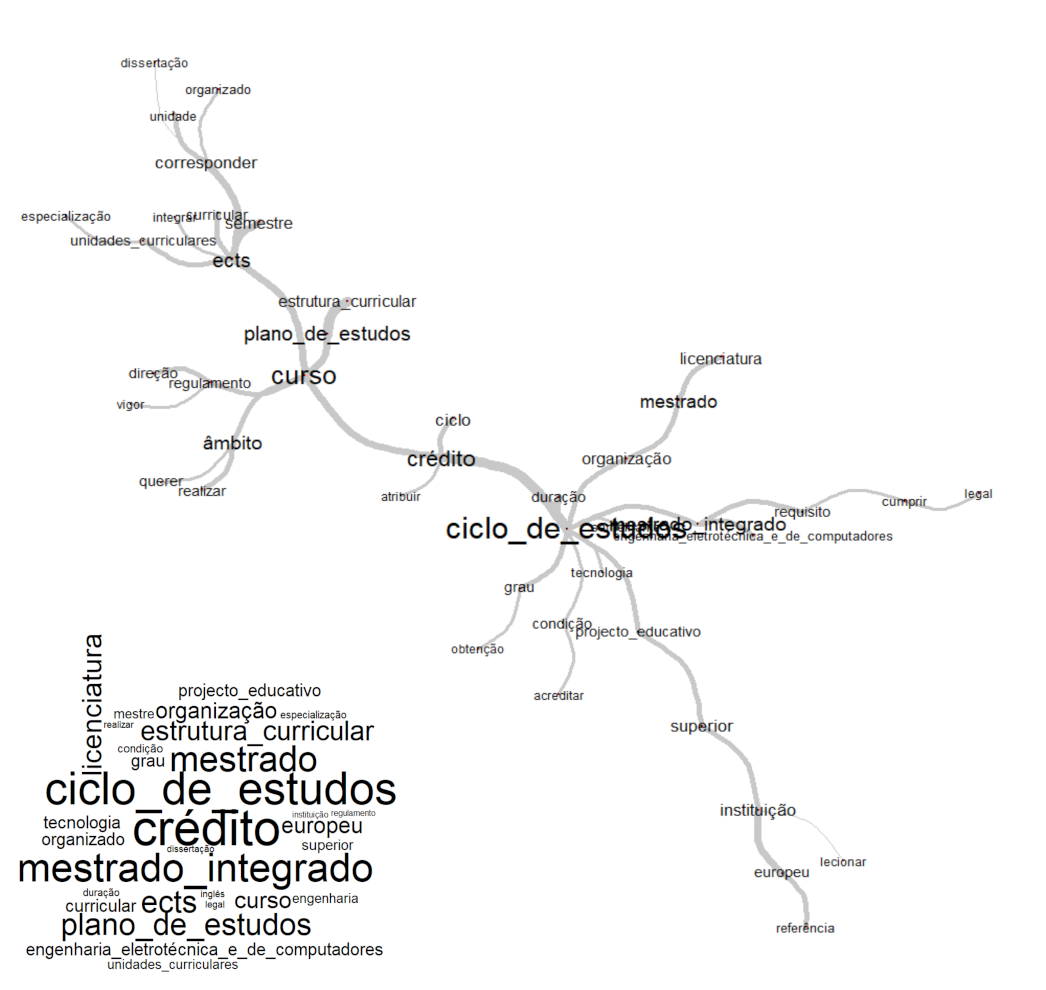
\includegraphics[width=0.75\textwidth]{Fig05.png}
 \caption{Análise de Similaridade dos \textit{drivers} da adoção de novas metodologias.}
 \label{Fig05}
 \source{dos autores.}
\end{figure}

Esta ADS representa os principais termos do \textit{corpus} textual de análise utilizado no estudo, sendo possível afirmar que este grafo é a representação visual de todas as classes que emergiram da análise qualitativa. Nesta exposição, a nuvem de palavras ao lado esquerdo inferior destaca os \textit{drivers} e \textit{outcomes} organizacionais e individuais que foram identificados na \Cref{sec-mapeamento}. Este agrupamento de direcionadores foi organizado com base no processo de decisão da inovação e na teoria institucional, podendo ser conferido no grafo da ADS (\Cref{Fig05}).

\section{Conclusão}\label{sec-conclusao}
É amplamente reconhecida na literatura internacional a necessidade de aumento da qualidade dos cursos de engenharia Elétrica e de computadores, adequando a formação dos novos engenheiros às expectativas profissionais do mercado. Como caminho para o desenvolvimento e aplicação de melhorias na formação dos engenheiros, este estudo identificou, em um curso, os \textit{drivers} e \textit{outcomes} institucionais que podem atuar na adoção de novas metodologias para a área de engenharia Elétrica e de computadores.

A teoria do processo de decisão da inovação permitiu entender, no ambiente do ciclo de estudos, como estava ocorrendo este processo. Como apoio, a teoria institucional complementou esta lente de análise, por permitir a identificação das práticas isomórficas herdadas do mercado de ensino superior, que estiveram presentes no ciclo de estudos avaliado.

A abordagem metodológica baseada em \textit{mixed methods} permitiu a análise cruzada entre os diversos documentos institucionais, regulamentos, avaliação externa pela agência e a ótica da direção do curso. Os resultados foram agregados em duas classes de análise de conteúdo relevantes: Competências e conhecimentos esperados dos estudantes (Classe 2, no texto acima), e aspectos da formação em engenharia Elétrica e de computadores (Classe 5, no texto acima).   

Os \textit{drivers} “formação”, “desenvolvimento” e “competências” foram oriundos da Classe 2, e tiveram associação com as características organizacionais. A “formação” promovida pelo curso mostrou estar bastante avançada quanto ao processo de decisão de inovação, prestes a adentrar no processo de consolidação do conhecimento científico e tecnológico nas unidades curriculares do ciclo de estudos, sendo estes \textit{outcomes} os difusores da inovação no curso. O “desenvolvimento” foi marcado pelo desempenho e investigação no curso, (\textit{outcomes}) que se mostraram no mesmo patamar de cursos semelhantes atuantes no espaço europeu de ensino superior. As “competências” avaliadas têm permitido o desenvolvimento do ensino pelos docentes e a aquisição da aprendizagem pelos estudantes como seus \textit{outcomes}, estando em estágio avançado de decisão de inovação no curso, à margem da sua consolidação como difusor da inovação no curso.

Na Classe 5, os \textit{drivers} “ciclo de estudos” e “tecnologia” apresentaram características institucionais, enquanto o \textit{driver} “novo” obteve associação individual com o desejo de inovação do diretor do curso. A “tecnologia”, pelas próprias características da área do curso, mostrou-se como um arranjo institucional padronizado, seguindo o seu projeto educativo, os padrões institucionais de qualidade difundidos pelo espaço europeu de ensino superior. Como consequência disto, o “ciclo de estudos” apresentou-se legitimado perante a comunidade académica do país, com práticas isomórficas de referência na área, identificadas principalmente nas unidades curriculares do curso. O \textit{driver} “novo”, por sua vez, apareceu como característica individual da direção do curso, em fase de desenvolvimento, pois ainda está no estágio de persuasão. Notou-se alguma resistência por parte do corpo docente, pela idade avançada, que foi uma característica limitadora de seu desenvolvimento no curso. 

A “UC” foi uma anomalia da análise, devido à massiva adoção da Ficha de Unidade Curricular pelos docentes do curso. Não pôde deixar de ser aqui mencionada, por ser um elemento que ajudou no desenvolvimento e adoção de práticas isomórficas já consolidadas nos demais cursos da área pela Europa.  

Como limitações deste estudo, os \textit{drivers} e \textit{outcomes} aqui identificados, embora tenham sido baseados na maior generalidade possível de documentos analisados, diferente das demais análises identificadas na literatura, estes resultados assentam num curso individual. Como perspetiva para estudos futuros, estes achados podem ser objeto de teste de replicação nos demais cursos da mesma área de conhecimento.

\section{Agradecimentos}\label{sec-agradecimentos}
Este estudo teve apoio financeiro atribuído pela Comissão Europeia através de bolsa de estudos de doutorado aprovada pelo Projeto Euro-Brazilian Windows + (EBW+), no Programa Erasmus Mundus.

\printbibliography\label{sec-bib}

\end{document}
